\documentclass[letterpaper,10pt]{article}
\usepackage[utf8]{inputenc}
\usepackage{fullpage}
\usepackage[english]{babel}
\usepackage{amsmath}
\usepackage{caption}
\usepackage{subcaption}
\usepackage{graphicx}

\renewcommand{\arraystretch}{1.4}
\setlength{\parindent}{0cm}

\begin{document}

\noindent
\begin{flushright}
    \large\textbf{Miguel Alcón Doganoc} \\
    Combinatorial Problem Solving \\
    May 7, 2019
\end{flushright}

\noindent
{\huge{\textbf{Logic Synthesis}}}

\section{Variables}
Given the number of input signals $n$, the depth $d$, and the specification (truth table) of the logical circuit, I defined the following variables:
\begin{itemize}
    \item $\mathbf{c_{i}}:=$ ``Code of the node $i$'', for $i \in \{0,1,...,2^{d+1}-2\}$.
    \item $\mathbf{b_{i}^t}:=$ ``Boolean value of the node $i$ for the row $t$ of the truth table'', for $i \in \{0,1,...,2^{d+1}-2\}$ and $t \in \{0,1,...,2^n\}$.
\end{itemize}

For example, for a NOR-circuit that implements the functionality of an AND gate (see figure \ref{fig:original}), with $n = d = 2$, one possible solution for the variables $c_i$ and $b_i^0$, with $i \in \{0,1,...,6\}$, is shown in figures \ref{subfig:ci} and \ref{subfig:bit}, respectively.
\begin{figure}[hbtp]
    \centering
    \begin{subfigure}[b]{0.45\textwidth}
        \raisebox{18mm}{\begin{tabular}{c c | c | c}
            $x_1$ & $x_2$ & $y$ & $t$\\ \hline
            0 & 0 & 0 & 0 \\
            0 & 1 & 0 & 1 \\
            1 & 0 & 0 & 2 \\
            1 & 1 & 1 & 3 \\
        \end{tabular}}
    \end{subfigure}\hspace{-0.2\textwidth}
    \begin{subfigure}[b]{0.45\textwidth}
        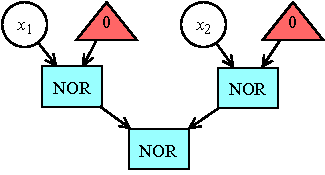
\includegraphics[width=\textwidth]{circuit.pdf}  
    \end{subfigure}
    \caption{Truth table of $y$ = AND($x_1,x_2$) and NOR-circuit implementing it.}
    \label{fig:original}
\end{figure}

\begin{figure}[hbtp]
    \centering
    \begin{subfigure}[b]{0.30\textwidth}
          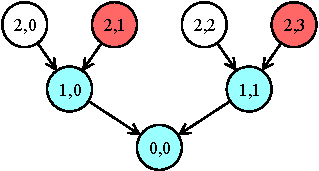
\includegraphics[width=\textwidth]{i.pdf}
          \caption{$i$}
          \label{subfig:i}
    \end{subfigure}
    \hspace{0.01\textwidth}
    \begin{subfigure}[b]{0.30\textwidth}
        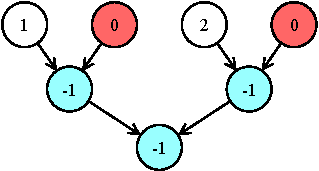
\includegraphics[width=\textwidth]{ci.pdf}
        \caption{$c_i$}
        \label{subfig:ci}
    \end{subfigure}
    \hspace{0.01\textwidth}
    \begin{subfigure}[b]{0.30\textwidth}
        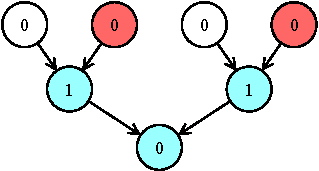
\includegraphics[width=\textwidth]{bit.pdf}
        \caption{$b_i^0$}
        \label{subfig:bit}
    \end{subfigure}
    \caption{Visual representation of some parameters and variables.}
    \label{fig:variables}
\end{figure}


\section{Constraints}
In order to simplify the definition of the constraints, I define two functions. Given the variable $x_i$, with $x_i = c_i$ or $b_i^t$,
\begin{itemize}
    \item \textbf{left($x_i$)} := ``Variable corresponding to the one on the left of $x_i$''
    \item \textbf{right($x_i$)} := ``Variable corresponding to the one on the right of $x_i$''
\end{itemize}

\end{document}